% !TEX program = XeLaTeX
\documentclass[11pt,a4paper,]{article}

% Fonts
\usepackage{libertine}
% This is a nice mathfont, it fits well with Libertine
% Comment the line if you want to use a different one
\usepackage[libertine]{newtxmath}
% The default monofont 
% Again, comment the line below if you want to change it
\usepackage[scaled=.95]{inconsolata}

% Add the following packages to support kableExtra
\usepackage{booktabs, longtable, makecell}
\usepackage{array}
\usepackage{multirow}
\usepackage{wrapfig}
\usepackage{colortbl}
\usepackage{pdflscape}
\usepackage{tabu}
\usepackage{threeparttable}
\usepackage{threeparttablex}
\usepackage[normalem]{ulem}
\usepackage{etoolbox}
\usepackage{tocloft}
\usepackage{rotating}
\usepackage{afterpage}
\usepackage{adjustbox}

% Dots in toc
\renewcommand{\cftsecleader}{\cftdotfill{\cftdotsep}}

% Colours
\usepackage[usenames,dvipsnames]{xcolor}
\definecolor{darkblue}{rgb}{0.0,0.0,0.55}

% Spacing
\usepackage{setspace}

% Margin
\usepackage[margin=2cm]{geometry}

% Packages I've been using for different reasons...
\usepackage{hyperref}
\usepackage{dcolumn}
\usepackage{graphicx}
\usepackage{float}
\floatplacement{figure}{H}
\usepackage{pgf}
\usepackage{tikz}
\usetikzlibrary{arrows}
\usetikzlibrary{positioning}
\usepackage{mathtools}
\usepackage{caption}

% UK English
\usepackage[UKenglish]{babel}
\usepackage[UKenglish]{isodate}
\cleanlookdateon

% Penalties
\exhyphenpenalty=1000
\hyphenpenalty=1000
\widowpenalty=1000
\clubpenalty=1000

% Hypersetup
\hypersetup{
  linkcolor=Mahogany,
  citecolor=Mahogany,
  urlcolor=darkblue, 
  breaklinks=true, 
  colorlinks=true,
      pdfauthor={Danilo Freire; Umberto Mignozzetti; Catarina Roman; Huzeyfe Alptekin},
      pdfkeywords={distributive politics; law of \(1/n\); legislature
size; meta-analysis; public spending},
  }

% If XeTex, LuaLaTeX, etc
\usepackage{ifxetex,ifluatex}
\usepackage{fixltx2e} % provides \textsubscript
\ifnum 0\ifxetex 1\fi\ifluatex 1\fi=0 % if pdftex
  \usepackage[T1]{fontenc}
  \usepackage[utf8]{inputenc}
\else % if luatex or xelatex
  \ifxetex
    \usepackage{amssymb,amsmath}
    \usepackage{mathspec}
  \else
    \usepackage{fontspec}
  \fi
  \defaultfontfeatures{Ligatures=TeX,Scale=MatchLowercase}
\fi
% use upquote if available, for straight quotes in verbatim environments
\IfFileExists{upquote.sty}{\usepackage{upquote}}{}
% use microtype if available
\IfFileExists{microtype.sty}{%
\usepackage{microtype}
\UseMicrotypeSet[protrusion]{basicmath} % disable protrusion for tt fonts
}{}

% Language

% Bibliography
\usepackage{natbib}
\bibliographystyle{apalike}
\makeatletter
% Remove comma after author
\setcitestyle{aysep={}}
\patchcmd{\NAT@citex}
	  {\@citea\NAT@hyper@{%
		 \NAT@nmfmt{\NAT@nm}%
		 \hyper@natlinkbreak{\NAT@aysep\NAT@spacechar}{\@citeb\@extra@b@citeb}%
		 \NAT@date}}
	  {\@citea\NAT@nmfmt{\NAT@nm}%
	   \NAT@aysep\NAT@spacechar\NAT@hyper@{\NAT@date}}{}{}
	\patchcmd{\NAT@citex}
	  {\@citea\NAT@hyper@{%
		 \NAT@nmfmt{\NAT@nm}%
		 \hyper@natlinkbreak{\NAT@spacechar\NAT@@open\if*#1*\else#1\NAT@spacechar\fi}%
		   {\@citeb\@extra@b@citeb}%
		 \NAT@date}}
	  {\@citea\NAT@nmfmt{\NAT@nm}%
	   \NAT@spacechar\NAT@@open\if*#1*\else#1\NAT@spacechar\fi\NAT@hyper@{\NAT@date}}
	  {}{}
% Patch case where name and year are separated by aysep
\patchcmd{\NAT@citex}
  {\@citea\NAT@hyper@{%
     \NAT@nmfmt{\NAT@nm}%
     \hyper@natlinkbreak{\NAT@aysep\NAT@spacechar}{\@citeb\@extra@b@citeb}%
     \NAT@date}}
  {\@citea\NAT@nmfmt{\NAT@nm}%
   \NAT@aysep\NAT@spacechar\NAT@hyper@{\NAT@date}}{}{}
% Patch case where name and year are separated by opening bracket
\patchcmd{\NAT@citex}
  {\@citea\NAT@hyper@{%
     \NAT@nmfmt{\NAT@nm}%
     \hyper@natlinkbreak{\NAT@spacechar\NAT@@open\if*#1*\else#1\NAT@spacechar\fi}%
       {\@citeb\@extra@b@citeb}%
     \NAT@date}}
  {\@citea\NAT@nmfmt{\NAT@nm}%
   \NAT@spacechar\NAT@@open\if*#1*\else#1\NAT@spacechar\fi\NAT@hyper@{\NAT@date}}
  {}{}
\makeatother

% Listings

% Verbatim

% Tables

% Graphics

% Make links footnotes instead of hotlinks:
%  \setlength{\emergencystretch}{3em}  % prevent overfull lines
 \providecommand{\tightlist}{%
   \setlength{\itemsep}{0pt}\setlength{\parskip}{0pt}}
   
% Numbered sections
\setcounter{secnumdepth}{5}
% % % Redefines (sub)paragraphs to behave more like sections
% \ifx\paragraph\undefined\else
% \let\oldparagraph\paragraph
% \renewcommand{\paragraph}[1]{\oldparagraph{#1}\mbox{}}
% \fi
% \ifx\subparagraph\undefined\else
% \let\oldsubparagraph\subparagraph
% \renewcommand{\subparagraph}[1]{\oldsubparagraph{#1}\mbox{}}
% \fi
% \usepackage{booktabs}
\usepackage{longtable}
\usepackage{array}
\usepackage{multirow}
\usepackage{wrapfig}
\usepackage{float}
\usepackage{colortbl}
\usepackage{pdflscape}
\usepackage{tabu}
\usepackage{threeparttable}
\usepackage{threeparttablex}
\usepackage[normalem]{ulem}
\usepackage{makecell}
\usepackage{xcolor}

% Spacing
\doublespacing

% Title
\title{The Effect of Legislature Size on Public Spending:\\
A Meta-Analysis\thanks{Freire, Mignozzetti, and Roman contributed
equally to all parts of the manuscript. Alptekin helped collect data in
the early stages of the project. The authors thank Guilherme Duarte,
Robert Myles McDonnell, and David Skarbek for their constructive
feedback. We also thank Cedric Antunes, Luis Castro, Giovanna França,
Julia Oriente, and Lucas Mingardi for their excellent research
assistance. Replication materials are available at
\url{https://github.com/danilofreire/legislature-size-meta-analysis}. We
kindly acknowledge funding from the São Paulo State Science Foundation
(FAPESP grant number 2018/00646-1).}}

% Author
\author{Danilo Freire\footnote{Senior Lecturer, School of Social and
  Political Sciences, University of Lincoln,
  \href{mailto:dfeire@lincoln.ac.uk}{\nolinkurl{dfeire@lincoln.ac.uk}},
  \url{https://danilofreire.github.io}.} \and Umberto
Mignozzetti\footnote{Visiting Assistant Professor, Quantitative Theory
  and Methods Department, Emory University,
  \href{mailto:umberto.mignozzetti@emory.edu}{\nolinkurl{umberto.mignozzetti@emory.edu}},
  \url{http://umbertomig.com}. Corresponding author.} \and Catarina
Roman\footnote{PhD Student, University of California, San Diego,
  \href{mailto:acroman@ucsd.edu}{\nolinkurl{acroman@ucsd.edu}},
  \url{http://catarinaroman.github.io}.} \and Huzeyfe
Alptekin\footnote{Independent Researcher,
  \href{mailto:huzeyfealptekin@gmail.com}{\nolinkurl{huzeyfealptekin@gmail.com}}.}}

% Date
\date{\today}

% Begin document
\begin{document}
\maketitle

% Abstract
\begin{abstract}
\doublespacing \noindent In a seminal article,
\citet{weingast1981political} argue that there is a positive
relationship between legislature size and inefficiency in public
expenditures. Their proposition is currently known as the ``law of
\(1/n\)'' and has been widely debated in political science and public
administration. However, recent studies have questioned the validity of
the theory. In this letter, we conduct the first meta-analysis that
assesses the generality of the ``law of \(1/n\)''. Based on a sample of
30 articles, we find no robust evidence suggesting that legislature size
has either a positive or a negative effect on government budgets. Yet
the aggregate results mask considerable heterogeneity. Our findings
provide moderate support for the ``law of \(1/n\)'' in unicameral
legislatures and in upper houses, but they also indicate that papers
using panel/fixed-effects models or regression discontinuity designs
report negative public spending estimates. We find only limited evidence
that electoral systems impact public spending, which suggests that
proportional representation systems may not be more prone to
overspending than majoritarian ones.
\vspace{.25cm}

\noindent \textbf{Keywords}: distributive politics; law of \(1/n\);
legislature size; meta-analysis; public spending
\vspace{.25cm}

\noindent \textbf{JEL Classification Codes}: H21; H23; H50; H61
\end{abstract}


% Table of Contents
\newpage

\hypertarget{introduction}{%
\section{Introduction}\label{introduction}}

\label{sec:intro}

Over the past decades, a large literature has examined the relationship
between legislature size and public expenditure.
\citet{weingast1981political} provided the general framework to analyse
distributive politics. The authors argue that the larger the number of
legislative districts (\(n\)), the smaller the share of tax burden each
one will bear (\(1/n\)), thus legislators have an incentive to overspend
in their districts and transfer the costs to the entire polity. Early
studies that empirically tested the ``law of \(1/n\)'', as the theory is
currently known, indeed found a positive correlation between the number
of legislature seats and different measures of government spending,
although these first results were mainly based on US state legislatures
and the effect was often limited to one house
\citep[e.g.,][]{baqir2002districting, gilligan1995deviations, gilligan2001fiscal}.

Later research, however, has questioned the validity of the ``law of
\(1/n\)''. \citet{primo2008distributive} affirm that, due to spatial
spillovers, a collection of small districts can supply public goods more
efficiently than the central government. The authors conclude that a
``reverse law of \(1/n\)'' may hold, wherein a higher number of
legislators in small constituencies decrease the overall public
spending. Similarly, \citet{primo2006stop} and \citet{chen2007law} find
that lower and upper chambers may have mixed effects on government
spending, while \citet{petterssonlidbom2012size} argues that the impact
of larger chamber sizes is negative when using data from Finland and
Sweden.

Since many empirical tests of the ``law of \(1/n\)'' have produced
conflicting results, scholars have expanded this research agenda and
closely investigated how institutional factors condition the original
formulation of the theory. For instance, authors such as
\citet{crowley2019law} and \citet{pecorino2018supermajority} accurately
point out that collective action problems have been overlooked in the
literature, and recent findings indicate that bicameralism
\citep{maldonado2013legislatures}, intergovernmental competition
\citep{crowley2015local}, redistricting \citep{lee2018court}, and party
ideology \citep{bjedov2014impact} strongly influence the relationship
between seats and spending. Moreover, the literature has increasingly
applied causal inference methods to estimate the effect of the ``law of
\(1/n\)'', and in contrast to previous studies using panel data,
regression discontinuity designs generally indicate that more
legislators decrease public expenditures
\citep{debenedetto2018effect, hohmann2017effect, lewis2019legislature, petterssonlidbom2012size}.
In this respect, scholars have long been aware of the theoretical and
empirical limitations of the ``law of \(1/n\)'', and the proliferation
of new studies reflect a conscious attempt to assess the robustness of
the theory.

In this letter, we conduct the first meta-analysis that tests the
generality of the ``law of \(1/n\)''. We select 30 articles that use
quantitative methods to evaluate the impact of legislature size over
government spending across several dimensions. Our study sample mirrors
the diversity of the literature. We found articles that present a
positive association between the number of legislators and public
expenditures, others suggesting that such relationship is negative, and
yet others that claim that there is no correlation between them. Given
the volume and the disparity of the studies, we employ meta-analysis to
summarise the results. Meta-analysis provides a rigorous approach to
combine heterogeneous outcomes into a single estimation, and it allows
scholars to gain valuable insights from the aggregated data
\citep{cooper2019handbook, hedges1985statistical}. Meta-analysis can
also identify potential sources of study variability, enabling
researchers to assess threats to external validity and direct future
efforts into more promising areas of academic inquiry
\citep{doucouliagos2008democracy}. Research synthesis methods have been
successfully applied in medicine and psychology since the 1970s
\citep{glass2015meta}, and our work contributes to the burgeoning
literature that uses meta-analytic methods to understand challenging
questions in political science
\citep{costa2017responsive, doucouliagos2008democracy, green2013field, lau2007effects, schwarz2020supporting}.

Aggregate results indicate that legislature size has no significant
impact on public spending. Our main meta-analysis estimates show that
the overall effect is not statistically different from zero, thus
confirming the conflicting findings reported by the literature. However,
methodological choices partially explain these divergent results. When
we look only at articles that use regression discontinuity designs
(RDDs), all four papers included in our sample consistently report a
negative relationship between a higher number of legislators and public
expenditures. Our meta-regressions provide further evidence that study
designs significantly influence the results. Using a sample of 162
coefficients, we find that articles that use causal inference methods
report lower effects than those that use OLS, and that unicameralism is
associated with higher government expenditures.

\hypertarget{data-and-methods}{%
\section{Data and Methods}\label{data-and-methods}}

We compiled our study sample in three search rounds. In the first round,
we gathered data from three large academic databases (Scopus, Microsoft
Academic, and Google Scholar) and looked for studies that were written
in English and cited \citet{weingast1981political}, as it is the
foundational work in the literature on the ``law of \(1/n\)''. To ensure
that our sample was comparable, we only selected papers that used
quantitative methods to analyse
data\footnote{Since meta-analysis requires a single estimate per observation,
we excluded articles that use interaction terms or quadratic specifications of
our selected variables. Please refer to Section C in the Supplementary Material
for a detailed description of the selection procedure. We also included two
PRISMA (Preferred Reporting Items for Systematic Reviews and Meta-Analyses)
flow diagrammes \citep{liberati2009prisma} showing the number of resulting
papers after each review step.}. After this stage, we identified six
measurements that the literature often employs to quantify government
expenditure and legislature size. For government expenditure, our study
sample uses (i) public expenditure as a share of GDP; (ii) public
expenditure per capita; and (iii) the natural logarithm of public
expenditure per capita as its main variables of interest. In regards to
legislature size, the variables are (i) lower chamber size; (ii) natural
logarithm of lower chamber size; and (iii) upper chamber
size\footnote{There are a few important nuances concerning coding
of these variables. Unicameralism, for example, is captured both by lower
chamber size ($n = 7$) and by log lower chamber size ($n = 5$). Since much of
the literature estimates how institutional designs affect this relationship,
ours and many other articles use both lower and upper chamber sizes as main
explanatory variables. We did not find any article that used the natural
logarithm of upper chamber size in their models.}.

In the second round, we did not require articles to cite
\citet{weingast1981political} and used a keyword-based query on Google
Scholar to broaden the scope of the first search. The search string
contained terms strongly associated with the literature on the ``law of
\(1/n\)'' and it was as follows:
\texttt{("upper\ chamber\ size"\ OR\ "lower\ chamber\ size"\ OR\ "council\ size"\ OR\ "parliament\ size"\ OR\ "legislature\ size"\ OR\ "number\ of\ legislators"\ OR\ "legislative\ size")\ AND\ ("spending"\ OR\ "expenditure"\ OR\ "government\ size")}.
We again restricted the search to articles written in English which
employed quantitative methods. This search added two new results to our
sample \citep{coate2011government, debenedetto2018effect}, but neither
of them included variables beyond the six measures we had previously
identified. In the third search round, we looked into the personal
webpages of every author whom we had already included in our sample. The
purpose of this manual search was to assess whether there was any
working paper or unpublished manuscript that we had missed in the two
former queries. We did not find any new article that satisfied the
inclusion criteria in this search. The full list of excluded records is
available for online consultation in the replication materials.
Combined, the three searches produced a dataset of 30 studies as of the
10\textsuperscript{th} of March 2021. Table \ref{tab:papers} contains
the full list of articles we analyse in this paper.

\scriptsize
\begin{longtable}{>{\raggedright\arraybackslash}p{3.9cm}>{\centering\arraybackslash}p{1.5cm}>{\centering\arraybackslash}p{2cm}>{\centering\arraybackslash}p{2.3cm}>{\centering\arraybackslash}p{1cm}>{\centering\arraybackslash}p{2cm}>{\centering\arraybackslash}p{1.1cm}}
\caption{Papers Included in the Meta-Analysis, Ordered by Year of Appearance}\\
\toprule
\raggedright Author(s) & \centering Journal & \centering Country & \centering Dependent Variable & \centering Method & \centering Institutional Design & \centering Electoral System
\tabularnewline
\midrule
\endfirsthead
\caption{Papers Included in the Meta-Analysis, Ordered by Year of Appearance (\textit{Continued})}\\
\toprule
\raggedright Author(s) & \centering Journal & \centering Country & \centering Dependent Variable & \centering Method & \centering Institutional Design & \centering Electoral System
\tabularnewline
\midrule
\endhead
Stein et al. (1998) & Unpub & Multiple (26) & PCTGDP & OLS & Mixed & NM \\ [0.5ex] 
Baqir (1999) & Unpub & USA & logExpPC & OLS & Unicameral & M \\ [0.5ex] 
Bradbury and Crain (2001) & JPubE & Multiple (37) & ExpPC, PCTGDP & PANEL & Mixed & NM \\ [0.5ex] 
Gilligan and Matsusaka (2001) & NTJ & USA & ExpPC & PANEL & Bicameral & M \\ [0.5ex] 
Baqir (2002) & PC & USA & logExpPC & OLS & Unicameral & M \\ [0.5ex] 
Ricciuti (2003) & Unpub & Multiple (23) & ExpPC & PANEL & Mixed & NM \\ [0.5ex] 
Mukherjee (2003) & CPS & Multiple (110) & PCTGDP & PANEL & Mixed & NM \\ [0.5ex] 
Lledo (2003) & Unpub & BRA & PCTGDP & PANEL & Unicameral & NM \\ [0.5ex] 
Ricciuti (2004) & RivPE & Multiple (75) & PCTGDP & OLS & Mixed & NM \\ [0.5ex] 
Matsusaka (2005) & SPPQ & USA & ExpPC & IV & Bicameral & M \\ [0.5ex] 
Primo (2006) & E\&P & USA & ExpPC & PANEL & Bicameral & M \\ [0.5ex] 
Erler (2007) & PC & USA & ExpPC, PCTGDP & PANEL & Bicameral & M \\ [0.5ex] 
Chen and Malhotra (2007) & APSR & USA & ExpPC & PANEL & Bicameral & M \\ [0.5ex] 
Fiorino and Ricciuti (2007) & PC & ITA & ExpPC & IV & Unicameral & NM \\ [0.5ex] 
MacDonald (2008) & PC & USA & logExpPC & OLS & Unicameral & M \\ [0.5ex] 
Schaltegger and Feld (2009) & JPubE & CHE & ExpPC & PANEL & Unicameral & NM \\ [0.5ex] 
Coate and Knight (2011) & AEJ & USA & logExpPC & OLS & Unicameral & M \\ [0.5ex] 
Pettersson-Lidbom (2012) & JPubE & FIN \& SWE & logExpPC & RDD & Unicameral & NM \\ [0.5ex] 
Baskaran (2013) & EJPE & DEU & ExpPC & IV & Unicameral & NM \\ [0.5ex] 
Maldonado (2013) & SSQ & Multiple (92) & PCTGDP & OLS & Mixed & NM \\ [0.5ex] 
Kessler (2014) & JPE & USA & ExpPC & PANEL & Unicameral & M \\ [0.5ex] 
Bjedov et al. (2014) & PC & CHE & ExpPC, PCTGDP & PANEL & Unicameral & NM \\ [0.5ex] 
Lee (2015) & PC & USA & ExpPC & IV & Bicameral & M \\ [0.5ex] 
Lee (2016) & PC & USA & ExpPC & IV & Bicameral & M \\ [0.5ex] 
Drew and Dollery (2017) & UAR & AUS & logExpPC & PANEL & Unicameral & NM \\ [0.5ex] 
Höhmann (2017) & PC & DEU & logExpPC & RDD & Unicameral & NM \\ [0.5ex] 
Lee and Park (2018) & PC & USA & ExpPC & PANEL & Bicameral & M \\ [0.5ex] 
De Benedetto (2018) & Unpub & ITA & logExpPC & RDD & Unicameral & NM \\ [0.5ex] 
Crowley (2019) & SEJ & USA & ExpPC & PANEL & Bicameral & M \\ [0.5ex] 
Lewis (2019) & SCID & IDN & logExpPC & RDD & Unicameral & NM \\ [0.5ex] 
\bottomrule
\label{tab:papers}
\begin{minipage}{\textwidth}
\renewcommand{\footnoterule}{}
\vspace{-0.5cm}
\scriptsize
\footnotetext{\scriptsize \textbf{Journal:} Unpub $=$ Unpublished, JPE $=$ Journal of Political
Economy, EJPE $=$ European Journal of Political Economy, PC $=$ Public Choice,
JPubE $=$ Journal of Public Economics, JPriE $=$ Journal of Private Enterprise,
APSR $=$ American Political Science Review, SEJ $=$ Southern Economic Journal,
UAR $=$ Urban Affairs Review, SCID $=$ Studies in Comparative International
Development, SSQ $=$ Social Science Quarterly, SPPQ $=$ State Politics and Policy
Quarterly, CPS $=$ Comparative Political Studies, RivPE $=$ Rivista di Politica
Economica, E\&P $=$ Economics and Politics, NTJ $=$ National Tax Journal.}
\footnotetext{\scriptsize \textbf{Country:} Country codes follow the ISO 3166-1 alpha-3
international standard.} 
\footnotetext{\scriptsize \textbf{Dependent Variable:} ExpPC $=$ Per capita expenditure,
logExpPC $=$ Natural logarithm of per capita expenditure, PCTGDP $=$ Expenditure as
a percentage of GDP.}
\footnotetext{\scriptsize \textbf{Method:} OLS $=$ Ordinary least squares, IV $=$ Instrumental
variables, Panel $=$ Panel data/fixed effects, RDD $=$ Regression discontinuity
design.}
\footnotetext{\scriptsize \textbf{Electoral System:} M $=$ Majoritarian, NM $=$ Non-majoritarian (mixed or proportional
representation).} 
\end{minipage} 
\end{longtable}
\normalsize

Our study sample reflects the development of the literature. Although
the ``law of \(1/n\)'' was first formulated in 1981, the empirical
assessment of the theory only started a few years later, as dates of
publishing range from 1998 to 2019. Most studies focus on the United
States (14), but our sample also contains papers on Australia (1),
Brazil (1), Germany (2), Indonesia (1), Italy (2), and Switzerland (2).
Seven articles use cross-national data and analyse from 2 to 110
countries. Early studies used OLS and panel data methods to estimate the
results, while studies from 2005 onward have also applied causal
inference models such as instrumental variables and regression
discontinuity designs to test the relationship between house size and
public spending.

Regarding the dependent variables included in the sample, 16 studies
employ public expenditure per capita, 9 papers use its natural
logarithm, and 8 of them analyse the impact of legislature size on
public expenditures as a percentage of GDP. This indicates that the area
has refined the original definition of the ``law of \(1/n\)'' and tested
the impact of larger legislatures on different measures of government
spending. Our independent variables are lower chamber size (26), the
natural logarithm of lower chamber size (7), and upper chamber size
(12). These variables formed a \(3 \times 3\) table, yet not all
combinations were available in the data. We found no studies that
correlate public expenditure per capita with either upper chamber size
or the natural logarithm of lower house size. Thus, our meta-analysis
contains seven of the nine possible variable combinations.

We also coded five moderators that may help us understand the
heterogeneity in the reported results. We included them in our
meta-regressions alongside an indicator for the type of independent
variable used in the original study. The additional moderators are: 1)
publication year; 2) paper publication in an academic journal; 3)
estimation method; 4) institutional design; 5) electoral system. Since
the literature on the ``law of \(1/n\)'' is notably diverse, we added
only moderators that either refer to important theoretical questions,
such as the effect of the electoral system on public spending, or to
essential characteristics of the publications themselves. Although more
moderators exist in the literature (e.g., data aggregation level), they
do not appear as often as necessary for their inclusion in the
meta-regressions. Table \ref{tab:descriptive} shows the descriptive
statistics of the moderator variables.

\vspace{.5cm}

\footnotesize

\begin{longtable}[t]{lcc}
\caption{\label{tab:descriptive}Descriptive Statistics of Moderators}\\
\toprule
  & Main Sample & Extended Sample\\
\endfirsthead
\caption[]{Descriptive Statistics of Moderators \textit{(continued)}}\\
\toprule
  & Main Sample & Extended Sample\\
\midrule
\endhead

\endfoot
\bottomrule
\endlastfoot
 & N=45 & N=162\\
\midrule
Independent Variables: &  & \\
\hspace{1em}Log of Lower Chamber Size & 7 (15.6\%) & 33 (20.4\%)\\
\hspace{1em}Lower Chamber Size & 26 (57.8\%) & 82 (50.6\%)\\
\hspace{1em}Upper Chamber Size & 12 (26.7\%) & 47 (29.0\%)\\
Year & 2009 (6.54) & 2008 (6.15)\\
Published work: &  & \\
\hspace{1em}No & 6 (13.3\%) & 17 (10.5\%)\\
\hspace{1em}Yes & 39 (86.7\%) & 145 (89.5\%)\\
Estimation method: &  & \\
\hspace{1em}OLS & 9 (20.0\%) & 49 (30.2\%)\\
\hspace{1em}PANEL & 25 (55.6\%) & 83 (51.2\%)\\
\hspace{1em}IV & 7 (15.6\%) & 19 (11.7\%)\\
\hspace{1em}RDD & 4 (8.89\%) & 11 (6.79\%)\\
Institutional Design: &  & \\
\hspace{1em}Bicameral & 17 (37.8\%) & 49 (30.2\%)\\
\hspace{1em}Mixed & 12 (26.7\%) & 50 (30.9\%)\\
\hspace{1em}Unicameral & 16 (35.6\%) & 63 (38.9\%)\\
Electoral system: &  & \\
\hspace{1em}Majoritarian & 22 (48.9\%) & 73 (45.1\%)\\
\hspace{1em}Non-Majoritarian & 23 (51.1\%) & 89 (54.9\%)\\*
\end{longtable}
\normalsize

A key methodological issue we had to address concerns the potential
violation of an important assumption in a meta-analysis, that of effect
size independence
\citep{cheung2014modeling, cheung2019guide, veroniki2016methods}. In our
study sample, authors frequently use the same datasets, and almost all
papers fit more than one regression with similar variables, what
suggests that the assumption above does not hold. We use two procedures
to tackle this problem. First, we created two sets of study coefficients
to reduce the impact of multicollinearity in our estimations. The first
group includes only the most rigorous models from each paper, that is,
those estimated with the largest \(n\), most control variables, and
fixed effects if the authors added them. If the article employed a
regression discontinuity design, we chose the coefficient from the
optimal bandwidth or from the intermediate one. This sample encompasses
45 estimates, as 13 articles analysed two dependent or independent
variables of interest\footnote{The papers that used more than one
dependent or independent variable of interest are \citet{bjedov2014impact,
bradbury2001legislative, chen2007law, crowley2019law, erler2007termlimits,
gilligan2001fiscal, lee2015supermajority, lee2016supermajority, lee2018court,
maldonado2013legislatures, primo2006stop, ricciuti2003trading,
ricciuti2004legislatures}.}. Our second sample, in contrast, contains
all the 162 effect sizes reported in the 30 papers. Here we focus on the
results for our restricted sample as we consider them more robust, but
the findings are nearly identical when we use the extended set.

Our second procedure consists of employing multilevel random effect
models \citep{cheung2014modeling, matthes2019meta} in all of our
estimations. We add two extra levels to the regular meta-analysis, the
first including a unique publication ID for each paper, and a second one
containing a common index for papers that share the same data
specifications. By adding these two levels, we account for within- and
between-study variation, thus removing these sources of effect size
dependency and improving the accuracy of the results. More information
about the multilevel models can be found in Section H.1 of the
Supplementary Material.

We use Hedges' \(g\) to calculate effect sizes in our meta-analysis
\citep{hedges1981distribution}. While there are other methods to
standardise coefficients in meta-analytic studies, Hedges' \(g\)
corrects for upward bias in small sample sizes and is considered more
robust than measures such as Cohen's \(d\)
\citep{lakens2013calculating}. We estimate the Standardised Mean
Difference (SMD), which represents the effect size in each study
relative to the variability observed in that study, by extracting the
coefficients and the standard errors from all articles included in our
sample and converting them to Hedges' \(g\). In cases where authors did
not report the standard errors for their estimates, we computed them
using the t-statistic presented in the original tables.

\hypertarget{results}{%
\section{Results}\label{results}}

The ``law of \(1/n\)'' states that more legislators increase government
expenditure. In this paper, we employ two methods to test the empirical
validity of that
relationship.\footnote{We also run preliminary binomial Z
tests in section G of the Supplementary Materials.} First, we fit nine
multilevel meta-analyses using the \texttt{meta}
\citep{balduzzi2019perform} and the \texttt{dmetar} \citep{dmetar2019}
packages for the \texttt{R} statistical language \citep{rstats2019}.
Then, we run four sets of meta-regressions to measure the effects of a
group of moderators on the effect sizes of our study sample. To
recapitulate, our independent variables of interest are lower chamber
size, the natural logarithm of lower chamber size, and upper chamber
size. The dependent variables are public expenditure per capita, the
natural logarithm of public expenditure per capita, and government
expenditure as a percentage of GDP. Since the outcomes have different
scales, we treat them separately in our models.

\hypertarget{meta-analysis}{%
\subsection{Meta-Analysis}\label{meta-analysis}}

\label{sub:Meta-Analysis}

We begin with the meta-analysis. We matched the house size variables
with our measures of government spending and created a theoretical
\(3 \times 3\) matrix. Out of the nine variable combinations, we found
only seven in the article pool. Our sample does not contain any papers
that analyse the relationships between log lower chamber size and public
expenditure per capita, or between upper chamber size and the logarithm
of public expenditure per capita.

Figure \ref{fig:plots} shows the forest plots for our restricted sample,
which includes the 45 main coefficients of the 30 selected
papers.\footnote{Please refer to Sections H and I in the Supplementary
Material for full results regarding both samples.} On the left side of
the plots are the names of the study authors and paper publication year.
For unpublished studies, we included the first year the paper was
available online. The bars in the middle show the reported effect sizes
and the vertical lines indicate their average, weighted by standard
errors. The length of the lines represent the precision of the
estimates. The red line at the bottom of the figures displays the
overall effects plus their respective confidence intervals.

The uppermost row shows the results for lower chamber size in our
restricted sample. In the first model, which correlates lower house and
expenditure per capita, we find a standardised mean difference (SMD) of
0.022 and a standard error of 0.131 (figure 1.1, studies = 16, 95\% CI =
{[}-0.256; 0.299{]}, \(p\)-value = 0.87), so we cannot rule out that the
effect is zero. Indeed, the effect of lower chamber size on the other
two dependent variables is also null in statistical terms. When we
compare lower chamber size with log expenditure per capita, the overall
effect size is -0.031 and the standard error is 0.049 (figure 1.2,
studies = 4, 95\% CI = {[}-0.188; 0.127{]}, \(p\)-value = 0.58). The
impact of larger lower houses on government spending as a percentage of
GDP is also negligible (figure 1.3, studies = 6, SMD = - 0.006, 95\% CI
= {[}-0.0334; 0.021{]}, \(p\)-value = 0.563). The results are virtually
identical when we estimate the meta-analyses using our extended sample,
and all three coefficients are again statistically indistinguishable
from zero.

Next, we present the meta-analyses using the logarithm of lower house
size as an independent variable. The relationship between this variable
and the log of per capita expenditure is positive, but the coefficient
is not significant (figure 1.4, studies = 5, SMD = 0.078, SE = 0.109,
95\% CI = {[}-0.225; 0.381{]}, \(p\)-value = 0.515). The effect of log
lower house size on expenditure as a percentage of the GDP is negative,
but it is again non-statistically significant (figure 1.5, studies = 2,
SMD = -1.576, SE = 2.223, 95\% CI = {[}-29.82; 26.668{]}, \(p\)-value =
0.607). Results in the full sample are also null, and the coefficients
for each dependent variable have the same sign as the restricted sample
-- positive and negative, respectively.

\begin{landscape}
\begin{figure}[!ht]
\centering
\caption{Forest Plots of the Relationship between Legislature Size and Government Spending (Main Sample)}
\vspace{0.3cm}
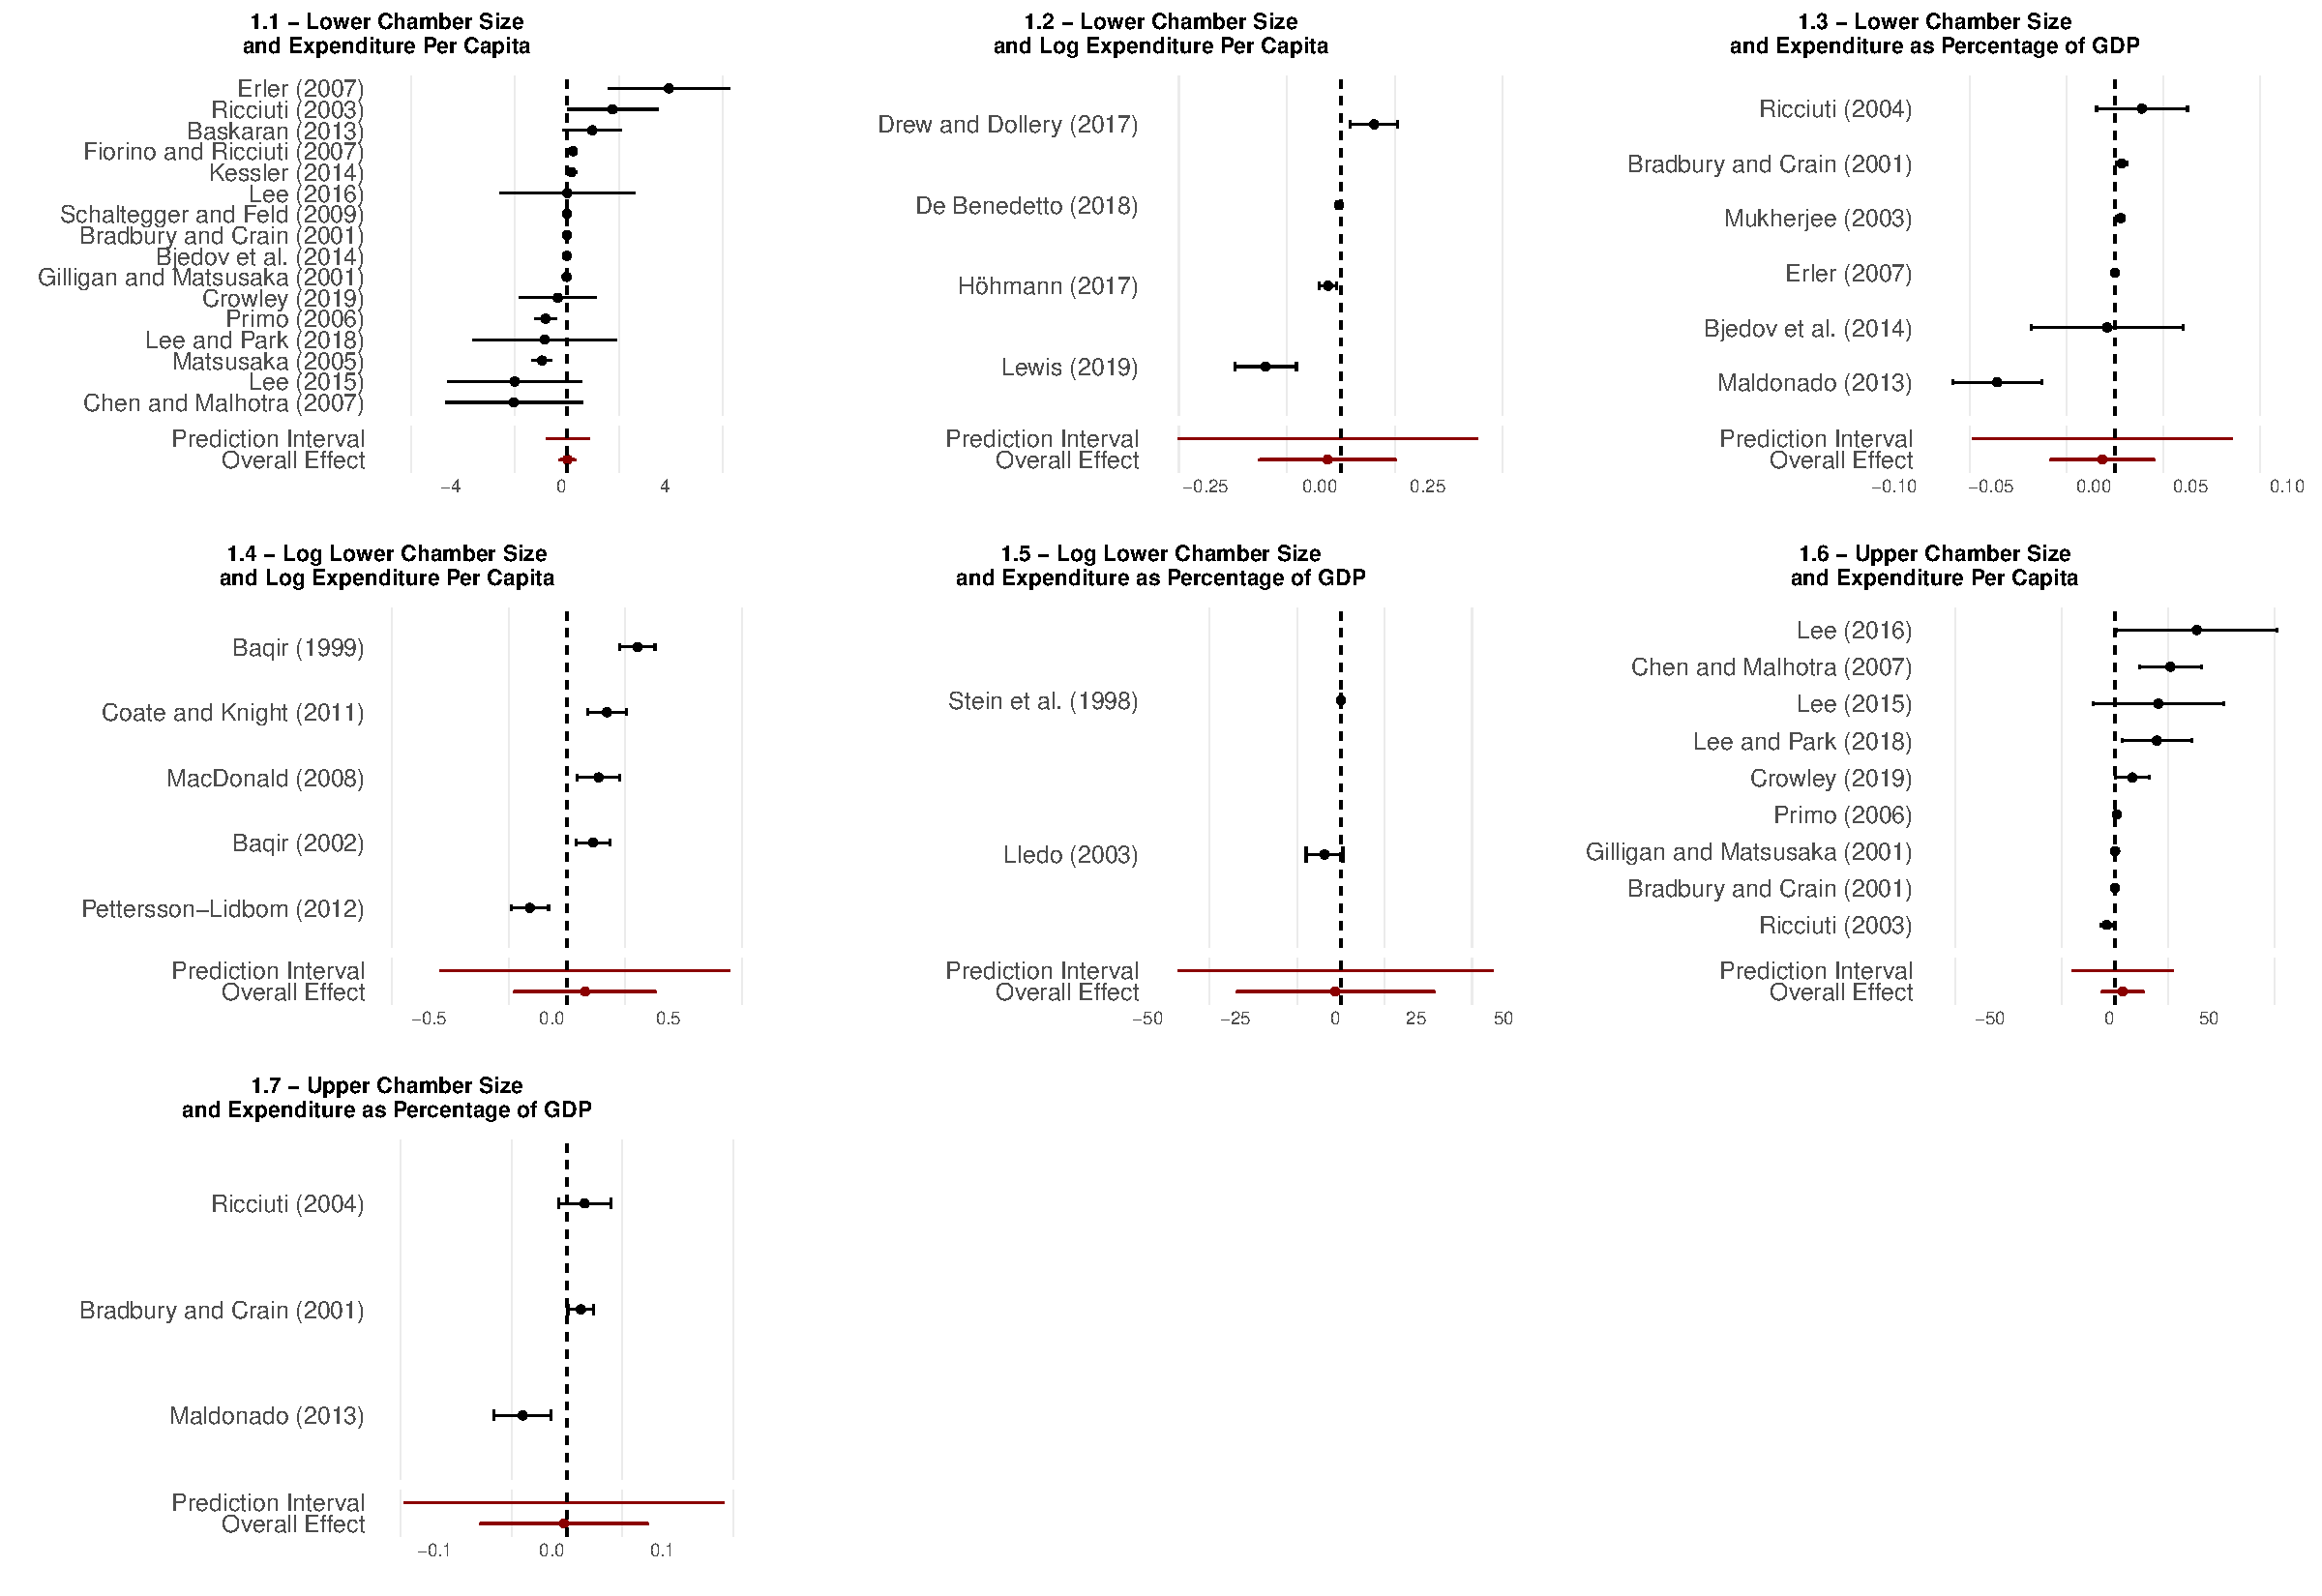
\includegraphics[width=25cm,height=17cm]{../graphs/graph1.pdf}
\label{fig:plots}
\end{figure}
\end{landscape}

The third set of models uses upper house size as the main independent
variable. We find a positive correlation between this variable and
expenditure per capita (figure 1.6, studies = 9, SMD = 3.658, SE =
4.299, 95\% CI = {[}-6.255; 13.572{]}, \(p\)-value = 0.419), and a
negative relationship with government spending as a percentage of GDP
(figure 1.7, studies = 3, SMD = -0.003, SE = 0.018, 95\% CI = {[}-0.079;
0.074{]}, \(p\)-value = 0.891), yet neither coefficient is statistically
significant. Results are the same in our extended sample.

Taken together, these results yield conservative interpretations.
Besides all average effect sizes not reaching conventional levels of
statistical significance, the studies are also notably heterogeneous.
The \(I^2\) statistic quantifies the degree of heterogeneity among
studies. \citet{higgins2019cochrane} consider any \(I^2\) value above
75\% to indicate high heterogeneity, and the lowest \(I^2\) we find in
the restricted sample is 80.7\% (for the subset of upper chamber size
and per capita expenditure). Additionally, all prediction intervals
encompass zero. Therefore, we cannot reject the null hypothesis that the
effect size is zero in any variable combination.

In a nutshell, we do not find evidence in favour of the ``law of
\(1/n\)''. One reason for this may be the identification strategy
authors use in their models. On the one hand, OLS and panel data models
require too many controls to make units comparable, and they are
vulnerable to omitted variable bias or post-treatment bias
\citep{cinelli2020making, pearl2015conditioning}. On the other hand,
estimation methods such as instrumental variables (IV) and regression
discontinuity designs (RDD) have become popular because of their high
internal validity \citep{angrist2008mostly}. Figure \ref{fig:plots2}
shows the disaggregated effects for two sets of models that employ
causal estimation techniques. They measure the impact of lower house
size on expenditure per capita (left) and on the natural logarithm of
expenditure per capita (right).

\vspace{.5cm}

\begin{figure}[htb]
\begin{center}
\caption{Forest Plots of the Relationship between Legislature Size and Government Spending with Regression Method Heterogeneity (Main Sample)}
\vspace{.3cm}
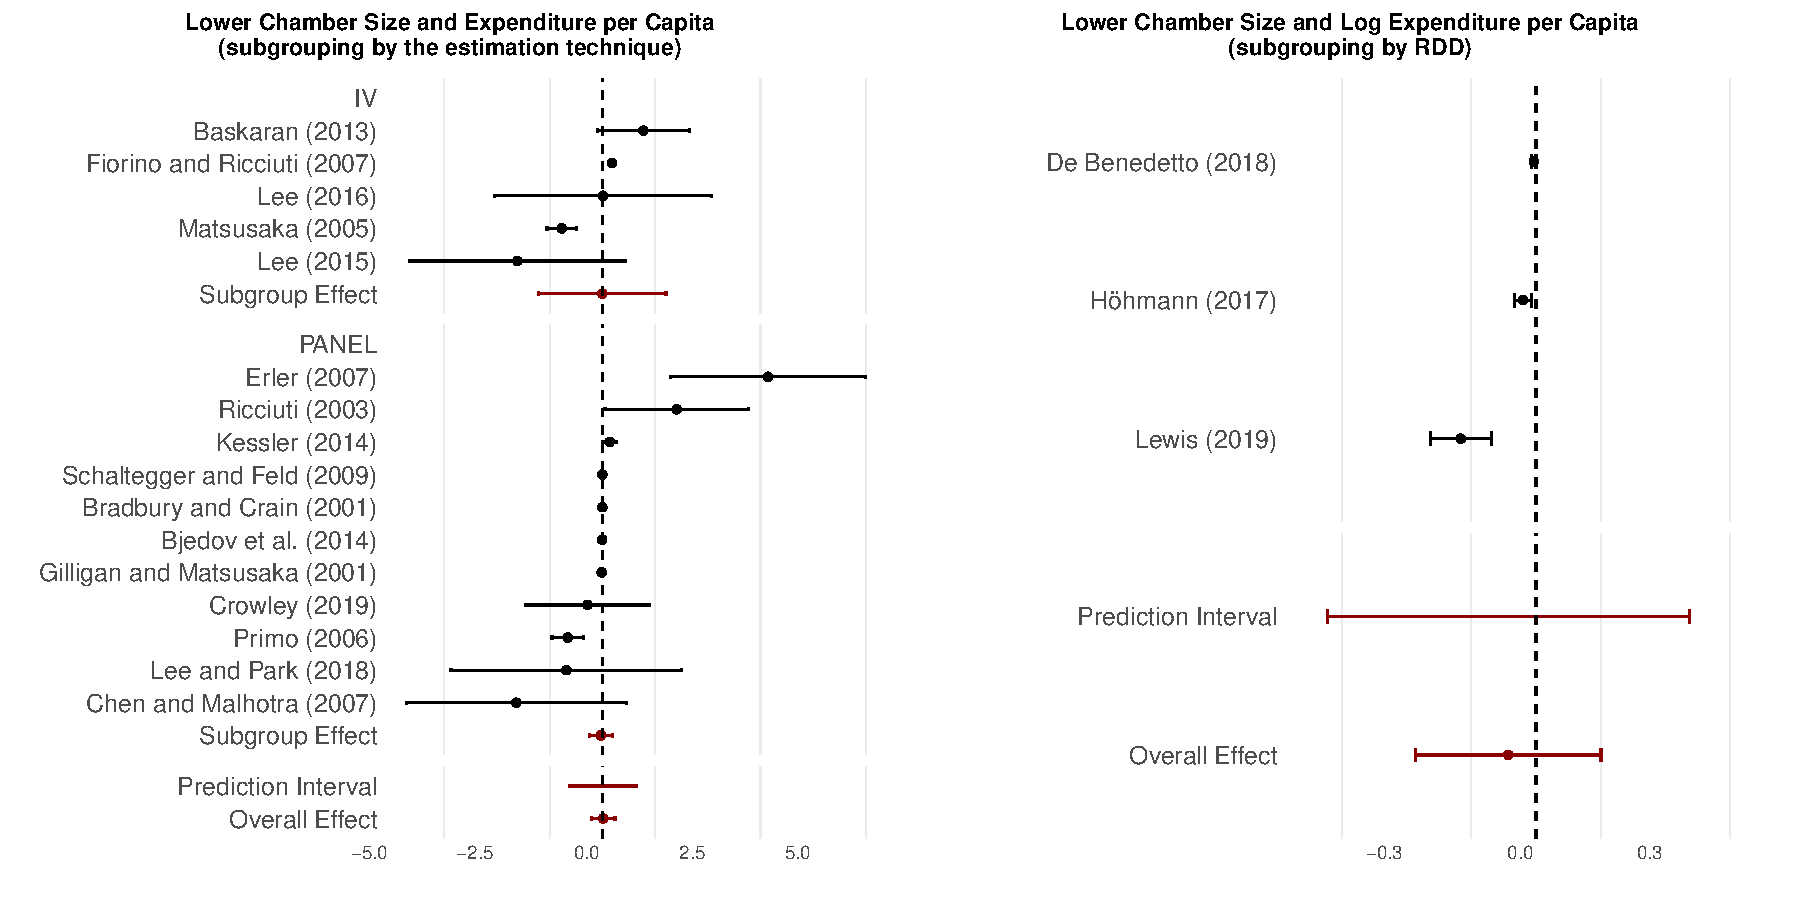
\includegraphics[width=1\linewidth, height=7.8cm]{../graphs/graph2.pdf}
\label{fig:plots2}
\end{center}
\end{figure}

Papers that employ instrumental variables and panel/fixed-effects models
show somewhat symmetrical distributions. Out of the five papers listed
under IV, two are positive, two are negative, and one is null. In the
plot for panel data, although more studies accumulate negative
coefficients, the positive shifts are more pronounced, so the overall
effect is also null. In contrast, all papers that use regression
discontinuity designs show negative and statistically significant
results. Since only three papers in this model use RDDs\footnote{\citet{petterssonlidbom2012size}
  also uses RDDs but the study is not included in this model as it
  employs log lower chamber size as the independent variable.}, we are
cautious about predicting an overall negative relationship, but they do
indicate that better identification strategies yield a zero-to-negative
impact of legislature size on expenditure, in support of the ``reverse
law of \(1/n\)''.

\hypertarget{meta-regressions}{%
\subsection{Meta-Regressions}\label{meta-regressions}}

\label{sub:regressions}

In this section, we run a series of meta-regressions with six moderators
to account for the heterogeneity across the selected papers. The first
variable indicates whether the study uses lower chamber size, log lower
chamber size, or upper chamber size as a main explanatory variable. We
include separate effect sizes for upper and lower chamber sizes when
papers analysed both. The second variable shows the study publication
year, which we included to capture temporal variation in the study
coefficients. We also add a dummy variable to assess whether published
articles report effect sizes that are higher or lower than those from
working papers. The fourth variable measures whether studies focusing on
non-majoritarian electoral systems report coefficients that are smaller
or larger than those from majoritarian countries. The fifth covariate is
a categorical variable indicating the statistical procedure used in the
original models (panel data, instrumental variables, OLS, or regression
discontinuity design). In our last variable, we separate coefficients
produced from samples of unicameral or bicameral systems, and code
papers that analyse multiple polities with different institutional
designs as ``mixed''.

Table \ref{tab:regressions} presents the meta-regression results for our
restricted and extended samples. Each column represents one of the three
measures of public spending we discuss in this paper, and the last one
uses all coefficients. To reduce the risk of false positives in our
analyses, we use permutation tests to calculate significance levels for
the meta-regressions \citep{higgins2004controlling}. To interpret these
results, the sign of coefficients matters the most. These
meta-regression coefficients can be viewed as representing ``the effect
of the moderator on the \(1/n\) effect''. This means positive
coefficients predict a strengthening of the \(1/n\) effect, and negative
ones predict it will get weaker under that moderator category, when
compared to its reference category. Since we aggregate different types
of independent variables under the same models, the size of the effects
does not accurately translate the scale of variations.

\vspace{0.5cm}

\begin{table}[htpb]
\caption{Meta-Regression Results\label{tab:regressions}}
\scriptsize
\centering
\begin{tabular}{lcccccccc}
\toprule
\midrule
\multicolumn{1}{c}{ } & \multicolumn{2}{c}{Expenditure Per Capita} & \multicolumn{2}{c}{Log Expenditure Per Capita} & \multicolumn{2}{c}{Gov. Spending \% GDP} & \multicolumn{2}{c}{All Coefficients} \\
\cmidrule(l{3pt}r{3pt}){2-3} \cmidrule(l{3pt}r{3pt}){4-5} \cmidrule(l{3pt}r{3pt}){6-7} \cmidrule(l{3pt}r{3pt}){8-9}
& Restricted & Extended & Restricted & Extended & Restricted & Extended & Restricted & Extended \\
\midrule
Log of Lower Chamber Size & 
 &  & 
-0.035 & -0.128 & 
-0.047 & -0.033 &
-0.222 & -0.148 \\
 &  &  & 
(0.134) & (0.124) & 
(0.028) & (0.024) & 
(0.144) & (0.090) \\
%
Lower Chamber Size &
-0.779 & -2.590*** & 
 &  & 
-0.009 & 0.002 &
-0.055 & -0.012 \\
 & (1.045) & (0.643) & 
 &  & 
(0.005) & (0.005) & 
(0.067) & (0.013) \\
%
Year & 
0.033 & 0.142** & 
0.000 & -0.005 & 
-0.007** & -0.006*** &
-0.013 & -0.001 \\
& (0.081) & (0.060) & 
(0.012) & (0.010) & 
(0.002) & (0.002) & 
(0.009) & (0.006) \\
%
Published: Yes & 
0.712 & 0.946 & 
-0.167* & 0.009 & 
 &  &
-0.084 & -0.009 \\
& (1.725) & (1.150) & 
(0.058) & (0.045) & 
 &  & 
(0.093) & (0.035) \\
%
Non-Majoritarian & 
0.455 & 0.819 & 
-0.300 & 0.006 & 
0.043 & 0.038* &
-0.082 & -0.190** \\
& (1.814) & (1.181) & 
(0.134) & (0.134) & 
(0.028) & (0.020) & 
(0.142) & (0.086) \\
%
Method: Panel & 
0.491 & -0.361 & 
0.200 & -0.354*** & 
-0.018 & -0.010 &
-0.027 & -0.137*** \\
& (0.975) & (0.977) & 
(0.104) & (0.050) & 
(0.017) & (0.013) & 
(0.114) & (0.032) \\
%
Method: IV & 
 & -0.565 & 
 & -0.052 & 
 &  &
-0.160 & -0.069** \\
&  & (0.894) & 
 & (0.050) & 
 &  & 
(0.190) & (0.034) \\
%
Method: RDD &
 &  & 
 & -0.308*** & 
 &  &
-0.168 & -0.200*** \\
&  &  & 
 & (0.041) & 
 &  & 
(0.147) & (0.036) \\
% 
Inst. Design: Mixed & 
-0.739 & -1.262 & 
 &  & 
-0.074* & -0.058*** &
0.123 & 0.192 \\
& (2.233) & (1.388) & 
 &  & 
(0.033) & (0.015) & 
(0.196) & (0.119) \\
% 
Inst. Design: Unicameral & 
-0.155 & -0.945 & 
 &  & 
 &  &
0.396** & 0.277** \\
& (1.718) & (1.000) & 
 &  & 
 &  & 
(0.162) & (0.115) \\
% 
Intercept & 
-67.291 & -282.761** & 
-0.030 & 10.432 & 
13.621** & 12.496*** &
26.032 & 2.505 \\
& (163.078) & (120.473) & 
(23.652) & (20.215) & 
(3.884) & (3.396) & 
(18.812) & (11.485) \\
\bottomrule
\end{tabular}
\begin{minipage}{\textwidth}
\renewcommand{\footnoterule}{}
\footnotetext{\textbf{Note:} {The restricted and extended samples include 45 and 162 study coefficients, respectively. We report the results from the permutation tests. Reference categories: Independent Variable $=$ Upper House Size; Published $=$ No; Method $=$ OLS, Inst. Design $=$ Bicameral. Significance codes: *** $p < 0.01$; ** $p < 0.05$; * $p < 0.10$. Blank cells mean that there is no sufficient data to estimate the parameter.}}
\end{minipage}
\end{table}

\vspace{0.5cm}

The first two models show the results for public expenditure per capita.
No variable reaches conventional levels of statistical significance in
the restricted sample. In the extended sample, we find that models that
use lower chamber size as an independent variable have lower effects
when compared to upper chamber size. This suggests that an additional
member in the lower house has a smaller impact on public spending than a
member in the upper house. Moreover, the results for the extended sample
point out that recent studies find larger effects than older ones.

The third and fourth columns use the natural logarithm of expenditure
per capita as the dependent variable. Among the coefficients in the
restricted sample, those in published studies tend to be smaller than
those in working
papers\footnote{We find no evidence of publication bias in our models.
The funnel plots for all estimations are available Sections H and I of the
Supplementary Material.}. Two other moderators are negatively associated
with the outcome in our larger coefficient pool. They both refer to
estimation methods. Studies that employ panel/fixed effects or
regression discontinuity designs (RDDs) have lower coefficients for log
expenditure per capita if we take OLS as the reference category.

Three estimates are statistically significant in the third set of
meta-regressions, which include public expenditure as a percentage of
GDP as the dependent variable. Both in our restricted and in our
extended samples, recent studies have smaller coefficients than older
papers, which stands in contrast with the first model. Institutional
design also affects outcomes. Papers that include both unicameral and
bicameral political systems report lower coefficients than those that
analyse bicameral exclusively. Non-majoritarian electoral systems have a
small, positive effect in our extended sample model, yet the coefficient
is only significant at the 10\% level.

The last two columns report meta-regressions that aggregate all selected
studies. In the restricted sample of coefficients, unicameralism has a
positive effect. This result holds for the extended sample as well. When
we regress all 162 coefficients, the effects of estimation methods
become stronger once again. Panel/fixed-effects models and regression
discontinuity designs both significantly decrease the \(1/n\) effect.
Instrumental variable models follow along these lines. Non-majoritarian
electoral systems are also significantly associated with lower levels of
public spending, which may be justified since the ``law of \(1/n\)'' was
conceived for majoritarian voting. These latter results, however, do not
replicate in the other sets of estimations.

The evidence seems to be sensitive to the methodological design. Our
results suggest that the same study samples may produce different
outcomes depending on the response variables scholars decide to analyse.
The broadest aggregation level presented the most insightful results in
dialogue with the literature. The additional legislator in
non-majoritarian legislatures does not increase expenditure as much as
she would if the system were majoritarian. We are also more likely to
witness legislative expenditure growing along with the amount of
representatives in unicameral legislatures rather than in bicameral
systems. This indicates that while the ``law of \(1/n\)'' is not
generalisable, its predicted effects are stronger when the institutional
features of a polity come closer to its original theoretical framework.

\hypertarget{discussion}{%
\section{Discussion}\label{discussion}}

\label{sec:discussion}

In this letter, we use meta-analytic methods to assess the generality of
the ``law of \(1/n\)''. Based on a sample of 30 publications, our
meta-analyses show that there is no strong evidence that more
legislators increase public expenditures. The meta-regressions indicate
that methodological considerations have a considerable influence on
reported results. In our extended sample, we find that modern inference
methods, such as RDDs, IVs and panel data yield lower coefficients than
OLS estimators. The models also indicate that unicameralism favours the
\(1/n\) effect. The remaining moderators show no consistent effects.

While the vast literature covering the ``law of \(1/n\)'' builds
important empirical knowledge, we hypothesise that some of the null
findings that we present here are due to difficulties in testing
important assumptions behind the theory itself. For instance, the theory
assumes three types of costs for legislative public good provision,
namely expenses for the constituency, expenses outside the constituency,
and externalities. The main issue in assessing their actual impact is
that externalities such as shifts in prices of local firms, for example,
are extremely hard to measure. Thus, it is very difficult to properly
translate the mechanism to empirical data, making it is easy to
accidentally distort results. Therefore, it should not come as a
surprise that slight differences in political features generate highly
heterogeneous results.

In this sense, the empirical cases in the literature may not always be
the most fortunate testing ground for the ``law of \(1/n\)''. While we
believe that moving beyond the majoritarian districts framework could
produce valuable insights, institutional features that are central to
the theory cannot be disregarded. For example, proportional
representation (PR) electoral systems allow candidates whose
constituents are spread across large territories to provide diffused
public goods and win elections. However, geographically-targeted service
provision is at the very core of the legislative behaviour that produces
the ``law of \(1/n\)''. Thus, scholars should consider the possible
implications of these micro-level dynamics when applying the ``law of
\(1/n\)'' logic to different settings.

Another plausible reason why there is no clear-cut evidence in favour or
against the ``law of \(1/n\)'' may be that there are few incentives for
the pure accumulation of knowledge in the social sciences, at least when
compared to the benefits scholars may accrue when they challenge or add
features to existing theories \citep{geddes2003paradigms}. This leads to
a reduced number of replication studies and research syntheses in the
field, although we have seen some positive changes in this respect, such
as EGAP's \emph{Metaketa Initiative}\footnote{See
\url{https://egap.org/our-work/the-metaketa-initiative} for further
information.}. Here we show that meta-analyses provide a viable path
towards knowledge-building in our discipline. Although aggregating
observational -- instead of experimental -- data can be especially
challenging, we believe that research synthesis methods play an
essential role in advancing our understanding of complex political
phenomena.

Our analyses suggest other avenues for further research. First, our
study sample did not include articles that evaluate the association
between the natural logarithm of lower chamber size and public
expenditure per capita, or between upper house size and log expenditure
per capita. New work on that area might clarify some of the
inconsistencies we find here. Second, despite the inclusion of several
moderators in our models, aggregate results still show considerable
heterogeneity. Domestic factors such as party dynamics or gerrymandering
\citep{lee2015supermajority, mukherjee2003politicalparties, gilligan2006public}
may prove useful in explaining those divergent results. Third, authors
should leverage natural and quasi-experiments to assess whether the
current results hold when systematically tested. Fortunately, this may
also be a trend under way, as all four studies using regression
discontinuity designs in our sample were published within less than 10
years prior to this meta-analysis. These suggestions may help scholars
to validate the robustness of their findings and policy-makers to reach
an optimal balance between sound fiscal policy and the demands for
increased political representation.

\hypertarget{backmatter-headings}{%
\section{Backmatter Headings}\label{backmatter-headings}}

\begin{itemize}
\item
  \textbf{Supplementary Materials}: The supplementary materials for this
  paper can be found at \url{https://URL_JOURNAL_HERE}.
\item
  \textbf{Data Availability Statement}: Replication data for this paper
  can be found at \url{https://doi.org/10.7910/DVN/5DEGYP}. Replication
  materials are also available at
  \url{https://github.com/danilofreire/legislature-size-meta-analysis}.
\item
  \textbf{Acknowledgements}: The authors thank Guilherme Duarte, Cathy
  Hafer, Robert Myles McDonnell, David Skarbek, and Howard Rosenthal for
  their constructive feedback. We also thank Cedric Antunes, Luis
  Castro, Giovanna França, Julia Oriente, and Lucas Mingardi for their
  excellent research assistance.
\item
  \textbf{Author Contributions}: Freire, Mignozzetti, and Roman
  contributed equally to all parts of the manuscript. Alptekin helped
  collect data in the early stages of the project.
\item
  \textbf{Financial Support}: We kindly acknowledge funding from the São
  Paulo State Science Foundation (FAPESP), grant number 2018/00646-1.
\item
  \textbf{Competing Interests}: None.
\end{itemize}

\newpage
\setlength{\parindent}{0cm}
\setlength{\parskip}{5pt}

\nocite{datasetCite, baskaran2013coalition, bradbury2009spatially, drew2017price,
erler2007termlimits, fiorino2007legislature, hohmann2017effect,
kessler2014communication, lewis2019legislature, lledo2003electoral,
mukherjee2003politicalparties, petterssonlidbom2012size, schaltegger2009large,
stein1998institutional, mukherjee2003politicalparties, macdonald2008impact,
matsusaka2005endogeneity, ricciuti2004legislatures, coate2011government}

% More bibliography
\bibliography{references.bib}

\end{document}
